\documentclass[a4paper, table]{article}
% Useful packages, sorted so packages of similar functionality are grouped together. Not all are essential to make the document work, however an effort was made to make this list as minimalistic as possible. Feel free to add your own!

% Essential for making this template work are graphicx, float, tabularx, tabu, tocbibind, titlesec, fancyhdr, xcolor and tikz. 

% Not essential, but you will have to debug the document a little bit when removing them are amsmath, amsthm, amssymb, amsfonts, caption, subcaption, appendix, enumitem, hyperref and cleveref.

% inputenc, lipsum, booktabs, geometry and microtype are not required, but nice to have.

\usepackage[utf8]{inputenc} % Allows the use of some special characters
\usepackage{amsmath, amsthm, amssymb, amsfonts} % Nicer mathematical typesetting
\usepackage{lipsum} % Creates dummy text lorem ipsum to showcase typsetting 

\usepackage{graphicx} % Allows the use of \begin{figure} and \includegraphics
\usepackage{float} % Useful for specifying the location of a figure ([H] for ex.)
\usepackage{caption} % Adds additional customization for (figure) captions
\usepackage{subcaption} % Needed to create sub-figures

\usepackage{tabularx} % Adds additional customization for tables
\usepackage{tabu} % Adds additional customization for tables
\usepackage{booktabs} % For generally nicer looking tables

\usepackage[nottoc,numbib]{tocbibind} % Automatically adds bibliography to ToC
\usepackage[margin = 2.5cm]{geometry} % Allows for custom (wider) margins
\usepackage{microtype} % Slightly loosens margin restrictions for nicer spacing  
\usepackage{titlesec} % Used to create custom section and subsection titles
\usepackage{titletoc} % Used to create a custom ToC
\usepackage{appendix} % Any chapter after \appendix is given a letter as index
\usepackage{fancyhdr} % Adds customization for headers and footers
\usepackage[shortlabels]{enumitem} % Adds additional customization for itemize. 

\usepackage{hyperref} % Allows links and makes references and the ToC clickable
\usepackage[noabbrev, capitalise]{cleveref} % Easier referencing using \cref{<label>} instead of \ref{}

\usepackage{xcolor} % Predefines additional colors and allows user defined colors

\usepackage{tikz} % Useful for drawing images, used for creating the frontpage
\usetikzlibrary{positioning} % Additional library for relative positioning 
\usetikzlibrary{calc} % Additional library for calculating within tikz

% Defines a command used by tikz to calculate some coordinates for the front-page
\makeatletter
\newcommand{\gettikzxy}[3]{%
  \tikz@scan@one@point\pgfutil@firstofone#1\relax
  \edef#2{\the\pgf@x}%
  \edef#3{\the\pgf@y}%
}
\makeatother



 % Loads in the preamble 
% Give your report a title
\newcommand\reporttitle{Trabajo de Planificación Ambiental de Proyectos}

% Insert course code, name, quartile number and year (or any other subtitle)
\newcommand\reportsubtitle{
Evaluación Ambiental de Proyectos
}

% Add your group number (for DBL) or any other text.
\newcommand\groupnumber{
\textbf{Group Number: C2566-OG0262-3476}
}

% Insert authors and student numbers here
\newcommand\reportauthors{
Isabela Arenas Escudero \\
Juan Pablo Tobón García \\
Juan Manuel Young Hoyos
}

% Add the name of your tutor (for DBL) or any other text.
\newcommand\grouptutor{
Tutor: Jose Alfredo Vasquez Paniagua
}

% Date and location (default: current date and Medellín)
\newcommand\placeanddate{
Medellín, \today
}

% Define EAFIT-blue (color of the EAFIT logo). Can be changed to drastically change the look of the template
\definecolor{EAFIT-blue}{RGB}{2, 8, 115}

% Sets up hyperlinks in the document to be colored
\hypersetup{
    colorlinks=true,
    linkcolor=EAFIT-blue,
    urlcolor=EAFIT-blue,
    citecolor = EAFIT-blue
    }
\urlstyle{same} % Defines settings for link and reference formatting

% Change bullet style for level 1, 2 and 3 respectively for itemize
\renewcommand{\labelitemi}{\scriptsize\textcolor{EAFIT-blue}{$\blacksquare$}}% level 1
\renewcommand{\labelitemii}{\scriptsize\textcolor{EAFIT-blue}{$\square$}}% level 2
\renewcommand{\labelitemiii}{\textcolor{EAFIT-blue}{$\circ$}}% level 3

% \renewcommand{\labelitemi}{\small\textcolor{EAFIT-blue}{\ding{70}}} % level 1
% \renewcommand{\labelitemii}{\small\textcolor{EAFIT-blue}{\ding{71}}}% level 2
% \renewcommand{\labelitemiii}{\tiny\textcolor{EAFIT-blue}{\ding{71}}}% level 3

% Change bullet style for level 1, 2 and 3 respectively for enumerate
\renewcommand{\labelenumi}{\textbf{\textcolor{EAFIT-blue}{\arabic*.}}}% level 1
\renewcommand{\labelenumii}{\textbf{\textcolor{EAFIT-blue}{[\alph*]}}}% level 2
\renewcommand{\labelenumiii}{\textbf{\textcolor{EAFIT-blue}{\roman*.}}}% level 3

% Have reference labels be linked to section (section 3 will have fig. 3.1 etc.)
\counterwithin{equation}{section} % For equations
\counterwithin{figure}{section} % For figures
\counterwithin{table}{section} % For tables

% Creates a beautiful header/footer
\pagestyle{fancy}
\lhead{
\includegraphics[height=14pt]{Figures/0. General/eafit_logo_blue.png}}
\rhead{\reporttitle}
\renewcommand{\footrulewidth}{0.4pt}
\cfoot{Page \thepage}

% Formats section, subsection and subsubsection titles respectively 
\titleformat{\section}{\sffamily\color{EAFIT-blue}\Large\bfseries}{\thesection\enskip\color{gray}\textbar\enskip}{0cm}{} % Formats section titles

\titleformat{\subsection}{\sffamily\color{EAFIT-blue}\large\bfseries}{\thesubsection\enskip\color{gray}\textbar\enskip}{0cm}{} % Formats subsection titles

\titleformat{\subsubsection}{\sffamily\color{EAFIT-blue}\bfseries}{\thesubsubsection\enskip\color{gray}\textbar\enskip}{0cm}{} % Formats subsubsection titles

% Formats captions
\DeclareCaptionFont{EAFIT-blue}{\color{EAFIT-blue}}
\captionsetup{labelfont={EAFIT-blue,bf}}

 % Changes font to mlmodern
\usepackage{mlmodern}

% Removes indent when starting a new paragraph
\setlength\parindent{0pt}

% Limits the ToC to sections and subsections (no subsubsec.)
\setcounter{tocdepth}{2}
 % Loads in user defined settings

% Paquetes para controlar la posición de tablas/figuras
\usepackage{placeins}   % \FloatBarrier

\begin{document}

% Portada
\begin{titlepage}

\centering

\begin{tikzpicture}

\node[opacity=0.3,inner sep=0pt,remember picture,overlay] at (4.5,-0.5){
    
\includegraphics[width=0.10\textwidth]{Figures/0. General/eafit_logo_gray.png}
};

\node[inner sep=0pt] (logo) at (0,0)
    {
\includegraphics[width=.25\textwidth]{Figures/0. General/eafit_logo_blue.png}};
    
\node[text width = 0.5\textwidth, right = of logo](title){\sffamily\huge\reporttitle};

\node[text width = 0.5\textwidth, yshift = 0.75cm, below = of title](subtitle){\sffamily\Large \reportsubtitle};

\gettikzxy{(subtitle.south)}{\sffamily\subtitlex}{\subtitley}
\gettikzxy{(title.north)}{\titlex}{\titley}
\draw[line width=1mm, EAFIT-blue]($(logo.east)!0.5!(title.west)$) +(0,\subtitley) -- +(0,\titley);

\end{tikzpicture}
\vspace{3cm}

\sffamily\groupnumber

\begin{table}[H]
\centering
\sffamily
\large
\begin{tabu} to 0.8\linewidth {cc}
\textbf{Nombre} & \textbf{Correo}\\
\hline

\sffamily\reportauthors

\end{tabu}

\end{table}

\sffamily \grouptutor

\tikz[remember picture,overlay]\node[anchor=south,inner sep=0pt] at (current page.south) {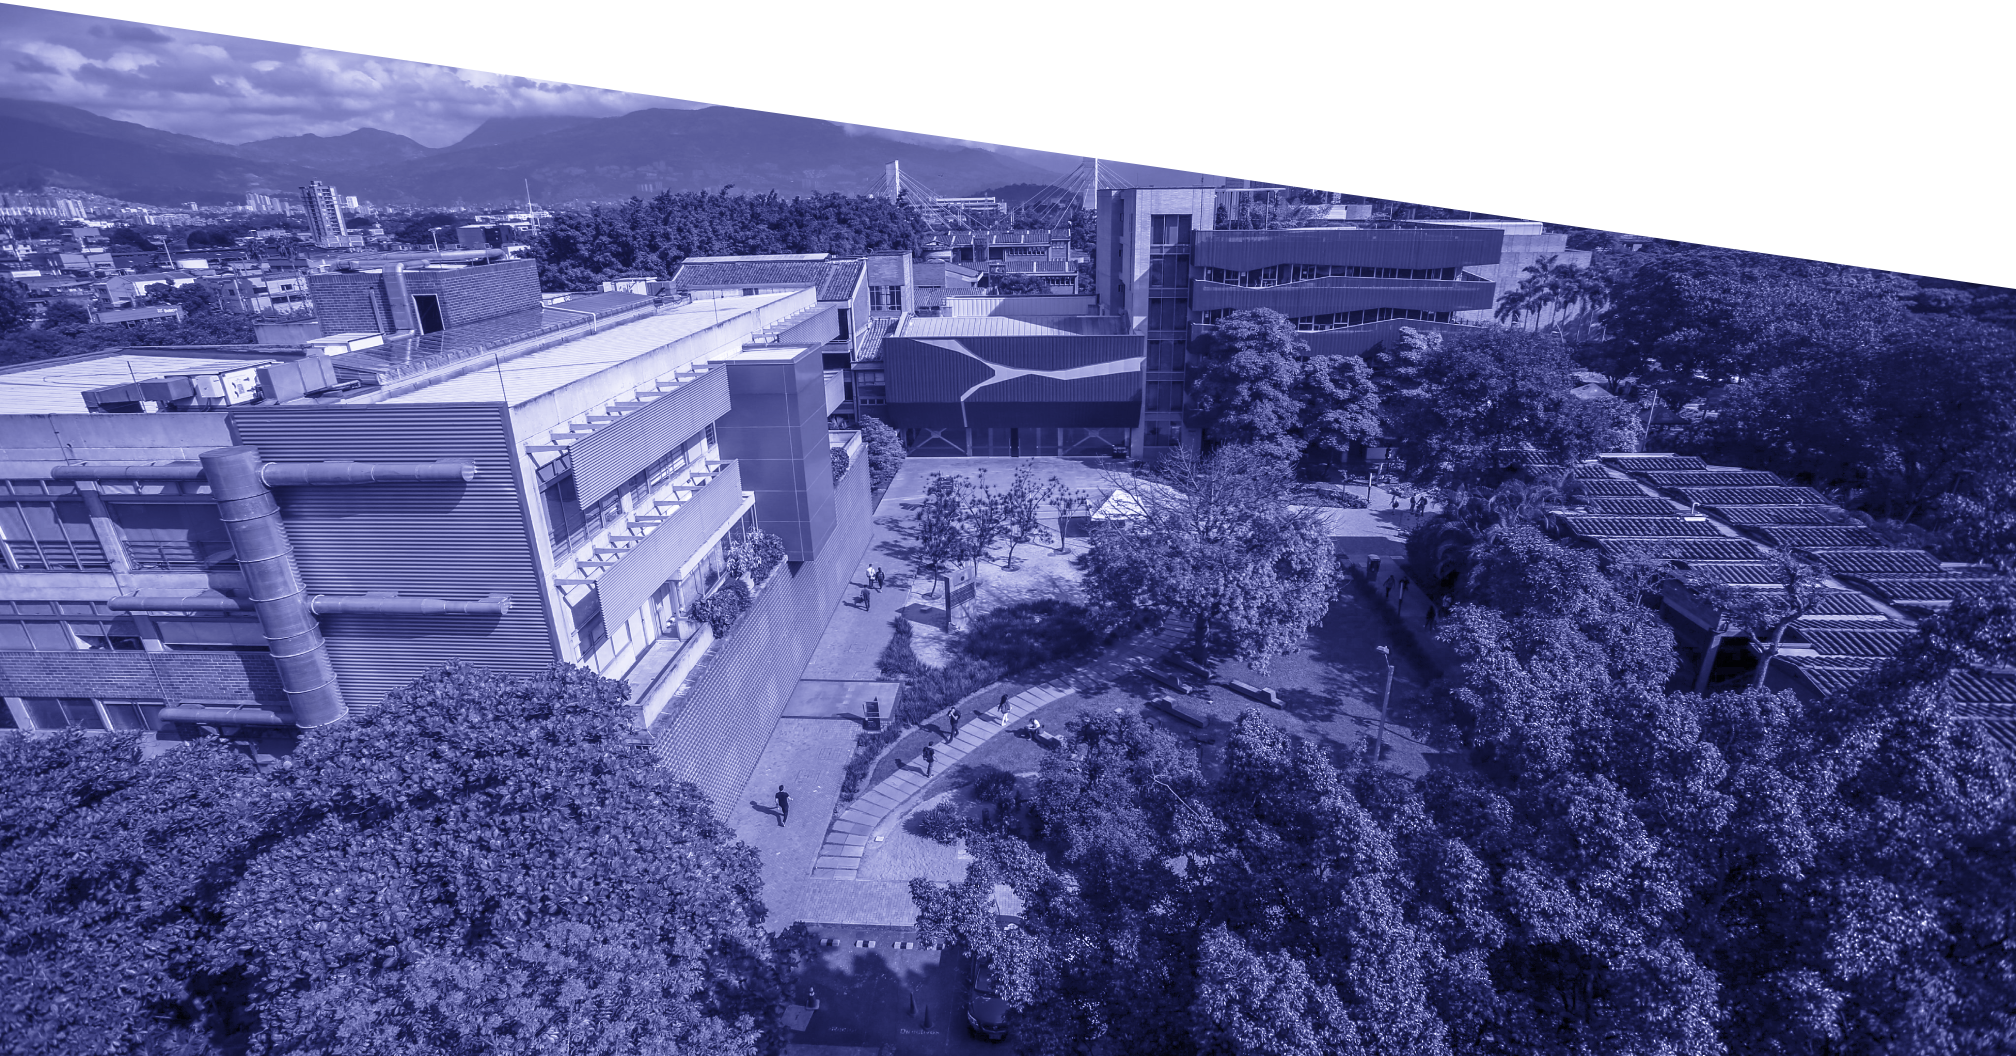
\includegraphics[width=\paperwidth]{Figures/0. General/eafit_banner.png}};

\mbox{}
\vfill
\sffamily \Large \textcolor{white}{\placeanddate} \\



\end{titlepage}








\pagenumbering{arabic}
\newpage

% Tabla de contenido
{\hypersetup{linkcolor=black}
\tableofcontents\thispagestyle{empty}}
\newpage

\section{Título del proyecto}
\textbf{Parque Solar Castilla (FV $\sim$21 MWp) — Planificación Ambiental en Preparación, Operación y Abandono}

\section{Resumen del proyecto}

El \textbf{Parque Solar Castilla} es una instalación fotovoltaica ubicada en el departamento del Meta, concebida para abastecer principalmente el \textit{Complejo Castilla} mediante un esquema de autogeneración con contrato interno (\emph{PPA}) entre el ancla de demanda y el operador. La capacidad instalada es del orden de \textbf{21 MWp}, con producción anual estimada acorde a la irradiancia del piedemonte llanero. El proyecto prioriza tiempos de construcción cortos y una reducción sustantiva de la huella de carbono frente a fuentes fósiles.

\medskip

\textbf{Alcance técnico:} módulos FV mono-PERC/bifaciales, estructuras fijas o seguidor (según optimización de LCOE), inversores \emph{string} o \emph{central}, subestación elevadora y SCADA para operación segura. Obras complementarias: cerramiento, vías internas, drenajes y gestión de escorrentía. En operación se privilegia \textit{uso eficiente del agua} o limpieza en seco; meta operativa de \textbf{cero vertimiento}.

\medskip

\textbf{Gestión ambiental:} el predio se selecciona evitando rondas hídricas, humedales y parches boscosos; se implementan medidas de \emph{control de erosión y sedimentos}, \emph{rescate y reubicación de fauna}, \emph{compensación forestal} cuando aplique, protocolo de \emph{hallazgo arqueológico}, y \emph{gestión integral de residuos} (ordinarios, \textsc{Raee} y \textsc{Respel}). El \textbf{Plan de Manejo Ambiental (PMA)} consolida programas de suelo, agua, aire/ruido, flora, fauna, social y arqueología, con indicadores e \textit{Informes de Cumplimiento Ambiental} (ICA) a la autoridad.

\medskip

\textbf{Competencia y permisos:} el instrumento rector es la \textbf{Licencia Ambiental} (\emph{licencia global}) que integra permisos asociados (aprovechamiento forestal, fauna, ocupación de cauce; concesión/vertimientos si aplica; emisiones sólo si hay fuentes fijas; plan arqueológico ante ICANH; residuos \textsc{Respel}/\textsc{Raee}). La autoridad competente será la \textbf{ANLA} por alcance/typología; si fuese de competencia regional en Meta, la autoridad sería \textbf{CORMACARENA}.

\medskip

\textbf{Cierre y abandono:} contempla retiro de módulos y estructuras, gestión de \textsc{Raee}/\textsc{Respel} con trazabilidad, reconformación y revegetalización de suelos, cumplimiento final de compensaciones y actos de terminación/cancelación de instrumentos (concesiones, vertimientos), hasta el \textit{paz y salvo} ambiental.

\medskip

\textbf{Marco normativo base (síntesis):} \textit{Ley 99 de 1993} (SINA; participación; inversión del 1\%), \textit{Decreto 2041 de 2014} (licenciamiento; incluye abandono), \textit{Decreto 1076 de 2015} (uso de recursos naturales; vertimientos; cauces; flora y fauna), \textit{Decreto 1541 de 1978} (concesiones de aguas), \textit{Decreto 3930 de 2010} y \textit{Resolución 631 de 2015} (vertimientos), \textit{Decreto 1791 de 1996} (forestal), \textit{Decreto 1608 de 1978} (fauna), \textit{Resolución 627 de 2006} (ruido), \textit{Decreto 948 de 1995} (aire), \textit{Ley 1185 de 2008}/ICANH (patrimonio), \textit{Decreto 4741 de 2005} (RESPEL), \textit{Ley 1715 de 2014} (FNCE).

\FloatBarrier

\section{FASE 1: Preparación -- Evaluación Ambiental}
\subsection{Identificación de impactos (Tabla A)}
\begin{table}[h]
\centering
\caption{Tabla A. Identificación de impactos ambientales}
\begin{tabular}{|l|p{10cm}|c|}
\hline
\textbf{Componente} & \textbf{Descripción de impactos ambientales} & \textbf{Calif.}\\ \hline
\multirow{3}{*}{Biótico} 
& Reducción puntual de cobertura vegetal por implantación de estructuras. & $-$\\
& Desplazamiento temporal de fauna durante construcción; rescate y reubicación. & $-$\\
& Microhábitats de sombra que favorecen especies pequeñas en operación. & $+$\\ \hline
\multirow{3}{*}{Atmosférico} 
& Reducción de emisiones de CO$_2$ por sustitución de generación fósil. & $+$\\
& Disminución de gases de combustión locales en operación. & $+$\\
& Polvo y ruido temporales por obra y tránsito de maquinaria. & $-$\\ \hline
\multirow{3}{*}{Hidrosférico} 
& Bajo consumo de agua comparado con otras tecnologías. & $+$\\
& Riesgo de arrastre de sedimentos por movimientos de tierra (obra). & $-$\\
& Mejora indirecta de calidad del agua por menor huella global de emisiones. & $+$\\ \hline
\multirow{3}{*}{Socioeconómico} 
& Generación de empleo directo e inclusión de mano de obra local. & $+$\\
& Programas con instituciones educativas (sensibilización/energía limpia). & $+$\\
& Tránsito y ruido temporal en comunidades aledañas durante obra. & $-$\\ \hline
\multirow{3}{*}{Cultural} 
& Sin afectación prevista a vestigios; protocolo de hallazgo fortuito. & $+$\\
& Promoción de cultura ambiental y tecnológica. & $+$\\
& Posible alteración menor por presencia de maquinaria. & $-$\\ \hline
\multirow{3}{*}{Paisaje} 
& Estructuras visibles que modifican la escena rural. & $-$\\
& Percepción positiva asociada a energías limpias. & $+$\\
& Integración con suelo productivo al no generar emisiones/olores. & $+$\\ \hline
\multirow{3}{*}{Geosférico} 
& Movimiento de tierras y compactación en frentes de obra. & $-$\\
& Protección frente a erosión por cobertura parcial y control de escorrentías. & $+$\\
& Alteración local por fundaciones y redes soterradas. & $-$\\ \hline
\end{tabular}
\end{table}

\subsubsection*{Sustento normativo}
Decreto 2041/2014 (licencias), Decreto 1076/2015 (gestión de recursos; programas de manejo), Resolución 631/2015 (vertimientos), Resolución 627/2006 (ruido), Decreto 1791/1996 (forestal), Decreto 1608/1978 (fauna), Ley 1185/2008 (patrimonio).

\FloatBarrier

\section{FASE 1: Preparación -- Uso de recursos naturales}
\subsection{Permisos, concesiones y autorizaciones (Tabla B)}
\begin{table}[h]
\centering
\caption{Tabla B. Uso de recursos naturales y restricciones}
\begin{tabular}{|l|l|p{8.6cm}|}
\hline
\textbf{Componente} & \textbf{Instrumento} & \textbf{Restricción / Condición}\\ \hline
Hidrosférico (captación) & Concesión de aguas (CORMACARENA o ANLA, según competencia) & Sólo si hay captación para limpieza; respetar caudal ecológico, medición y PUEAA. \\ \hline
Hidrosférico (vertimientos) & Permiso de vertimientos & Procede sólo si hay descarga; cumplir Res.\ 631/2015; meta preferible: \textit{cero vertimiento}.\\ \hline
Cauces & Permiso de ocupación de cauce & Para pasos/obras sobre drenajes; sin alterar régimen hídrico; restitución morfológica.\\ \hline
Atmosférico & Permiso de emisiones & Sólo si hay fuentes fijas (p.ej.\ grupo electrógeno permanente); cumplir límites.\\ \hline
Flora & Aprovechamiento forestal & Censo/acta de aprovechamiento y \textit{compensación} con mantenimiento.\\ \hline
Fauna & Plan de Manejo de Fauna & Rescate y reubicación previos; prohibición de caza/tenencia; reportes.\\ \hline
Patrimonio & PMA arqueológico / hallazgo fortuito (ICANH) & Parar obra, aislar, avisar; reanudación con concepto del ICANH.\\ \hline
Residuos & PGIRS y, si aplica, RESPEL/RAEE & Segregación, almacenamiento, transporte y gestor autorizado con manifiestos.\\ \hline
\end{tabular}
\end{table}

\subsubsection*{Sustento normativo}
D.\ 1541/1978 (concesiones), D.\ 3930/2010 y Res.\ 631/2015 (vertimientos), D.\ 1076/2015 (ocupación de cauce), D.\ 948/1995 (aire), D.\ 1791/1996 (forestal), D.\ 1608/1978 (fauna), Ley 1185/2008 (patrimonio), D.\ 4741/2005 (RESPEL).

\FloatBarrier

\section{FASE 2: Formulación y evaluación ambiental}
\subsection{Estudio sectorial y de mercado}
\textbf{Producto y cliente.} Autogeneración a gran escala para el complejo Castilla (PPA interno).\\
\textbf{Demanda/competencia.} Creciente penetración de FNCE; LCOE competitivo; tiempos de obra cortos.\\
\textbf{Riesgos sectoriales.} Variabilidad de irradiancia, degradación de módulos ($\sim$0.5\%/año), curtailment, cambios regulatorios.\\
\textbf{Fuentes.} Atlas de radiación (IDEAM/UPME), POT, demanda interna, capacidad de conexión.\\
\textbf{Norma base.} Ley 1715/2014; CREG 030/2018; Ley 142/1994.

\subsection{Estudio técnico y de localización}
\textbf{Criterios de emplazamiento.} Alta irradiancia; predio industrial; topografía suave; evitar rondas/fragmentos; conexión cercana.\\
\textbf{Diseño.} Módulos mono-PERC/bifaciales; estructuras fijas o seguidor; inversores; trafo elevador; SCADA; drenajes; control de polvo; plan antiincendios.\\
\textbf{Construcción.} Desbroce controlado; rescate de epífitas y fauna; acopios impermeabilizados; PGIRS/RESPEL; protocolo arqueológico.\\
\textbf{Operación.} Limpieza con uso eficiente de agua o en seco; meta \textit{cero vertimiento}; mantenimiento preventivo; control de vegetación.\\
\textbf{Norma base.} D.\ 1076/2015; Res.\ 631/2015; D.\ 1791/1996; D.\ 1608/1978; Ley 1185/2008; NSR-10; POT.

\subsection{Estudio administrativo}
\textbf{Gobernanza.} Titular, operador (HSE), interventoría ambiental, gestores autorizados; relación con Alcaldía, comunidad, ANLA/CORMACARENA, ICANH.\\
\textbf{Participación.} Socialización, mecanismo de PQRS, empleo local, compras locales, educación ambiental.\\
\textbf{Cronograma de referencia.} Prefactibilidad (6--9 m), factibilidad/licencia (6--12+ m), construcción (6--12 m), operación (15--30 a), abandono (3--12 m).\\
\textbf{Norma base.} Ley 99/1993; D.\ 2041/2014; D.\ 1072/2015.

\subsection{Estudio legal}
\textbf{Instrumento principal.} Licencia Ambiental (licencia global) integrando permisos asociados (forestal, fauna, cauce, concesión/vertimientos si aplican, aire si hay fuentes fijas, arqueología, residuos).\\
\textbf{Competencia.} ANLA por alcance/tipología; si fuere regional: CORMACARENA (Meta).\\
\textbf{Obligaciones típicas.} Ejecución del PMA, reportes y monitoreos, compensaciones, plan de abandono.\\
\textbf{Norma base.} D.\ 2041/2014; D.\ 1076/2015; D.\ 1541/1978; D.\ 3930/2010; Res.\ 631/2015; D.\ 1791/1996; D.\ 1608/1978; Res.\ 627/2006; D.\ 948/1995; Ley 1185/2008; D.\ 4741/2005.

\subsection{Estudio económico (costos ambientales)}
\begin{itemize}
\item \textbf{Planeación y licencias:} EIA/EMAS, trámites, estudios de suelo y biodiversidad, capacitaciones HSE.
\item \textbf{Implementación:} medidas de mitigación (polvo, ruido, escorrentías), revegetalización, drenajes, equipos de monitoreo.
\item \textbf{Operación:} monitoreo continuo (agua/ruido/aire), O\&M ambiental, personal, reportes.
\item \textbf{Compensaciones:} forestal y programas comunitarios.
\item \textbf{Abandono:} desmantelamiento, RAEE/RESPEL, restauración y evaluación final.
\end{itemize}

\subsection{Estudio financiero (supuestos y flujo)}
\subsubsection*{Parámetros clave}
\begin{table}[h]
\centering
\begin{tabular}{|l|r|l|}
\hline
\textbf{Parámetro} & \textbf{Valor} & \textbf{Justificación}\\ \hline
Inversión total & \$\,20{,}000{,}000 & CAPEX estimado del parque y conexión interna\\
Vida útil & 15 años & Horizonte del contrato y equipos principales\\
Ingreso año 1 & \$\,3{,}000{,}000 & PPA interno (producción $\times$ tarifa)\\
Crec.\ ingresos & 2\% anual & Indexación/IPC\\
OPEX año 1 & \$\,500{,}000 & O\&M, personal y seguros\\
Crec.\ OPEX & 3\% anual & Inflación/mant.\ preventivo\\
Degradación módulos & $-0.5$\% anual & Pérdida de performance\\
Plan de abandono & \$\,1{,}000{,}000 & Desmantelamiento y restauración\\ \hline
\end{tabular}
\end{table}

\subsubsection*{Flujo simplificado (0--15)}
\begin{table}[h]
\centering
\small
\begin{tabular}{|c|l|r|r|r|r|}
\hline
\textbf{Año} & \textbf{Concepto} & \textbf{Entradas} & \textbf{Salidas} & \textbf{Flujo} & \textbf{Acumulado}\\ \hline
0 & Inversión inicial y estudio & 0 & \$\,20{,}000{,}000 & -\$\,20{,}000{,}000 & -\$\,20{,}000{,}000\\
1 & EIA e inicio operación & \$\,3{,}000{,}000 & \$\,700{,}000 & \$\,2{,}300{,}000 & -\$\,17{,}700{,}000\\
2 & Operación & \$\,3{,}060{,}000 & \$\,515{,}000 & \$\,2{,}545{,}000 & -\$\,15{,}155{,}000\\
3 & Operación & \$\,3{,}121{,}200 & \$\,530{,}450 & \$\,2{,}590{,}750 & -\$\,12{,}564{,}250\\
4 & Operación & \$\,3{,}183{,}624 & \$\,546{,}364 & \$\,2{,}637{,}261 & -\$\,9{,}926{,}990\\
5 & Operación & \$\,3{,}247{,}296 & \$\,562{,}754 & \$\,2{,}684{,}542 & -\$\,7{,}242{,}447\\
6 & Operación & \$\,3{,}312{,}242 & \$\,579{,}637 & \$\,2{,}732{,}605 & -\$\,4{,}509{,}842\\
7 & Operación & \$\,3{,}378{,}487 & \$\,597{,}026 & \$\,2{,}781{,}461 & -\$\,1{,}728{,}381\\
8 & Operación & \$\,3{,}446{,}057 & \$\,614{,}937 & \$\,2{,}831{,}120 & \$\,1{,}102{,}739\\
9 & Operación & \$\,3{,}514{,}978 & \$\,633{,}385 & \$\,2{,}881{,}593 & \$\,3{,}984{,}332\\
10 & Operación & \$\,3{,}585{,}278 & \$\,652{,}387 & \$\,2{,}932{,}891 & \$\,6{,}917{,}223\\
11 & Operación & \$\,3{,}656{,}983 & \$\,671{,}958 & \$\,2{,}985{,}025 & \$\,9{,}902{,}248\\
12 & Operación & \$\,3{,}730{,}123 & \$\,692{,}117 & \$\,3{,}038{,}006 & \$\,12{,}940{,}254\\
13 & Operación & \$\,3{,}804{,}725 & \$\,712{,}880 & \$\,3{,}091{,}845 & \$\,16{,}032{,}099\\
14 & Operación & \$\,3{,}880{,}820 & \$\,734{,}267 & \$\,3{,}146{,}553 & \$\,19{,}178{,}652\\
15 & Operación + Abandono & \$\,3{,}958{,}436 & \$\,1{,}756{,}295 & \$\,2{,}202{,}141 & \$\,21{,}380{,}794\\ \hline
\end{tabular}
\end{table}
\textit{Nota:} valores ilustrativos consistentes con el cuadro de trabajo; puedes añadir VAN/TIR si tu tutor lo pide.

\FloatBarrier

\section{FASE 3: Operación — Obligaciones de la licencia y permisos}

\subsection{Obligaciones generales}
Ejecutar el \textbf{PMA} aprobado y actualizarlo si hay cambios sustanciales; garantizar pólizas y trazabilidad documental; presentar \textbf{Informes de Cumplimiento Ambiental} (ICA) en la periodicidad ordenada.\\
\textbf{Norma:} D.~2041/2014; Ley 99/1993.

\subsection{Suelo y manejo de escorrentía}
Delimitar áreas, estabilizar taludes, zanjas y disipadores de energía; control de erosión y sedimentos; revegetalización con nativas.\\
\textbf{Norma:} D.~1076/2015.

\subsection{Agua (captación/vertimientos)}
Concesión y medición si se capta; permiso y cumplimiento Res.~631/2015 si se descarga; \textbf{meta: cero vertimiento} con recirculación/reúso.\\
\textbf{Norma:} D.~1541/1978; D.~3930/2010; Res.~631/2015; D.~1076/2015.

\subsection{Aire y ruido}
Permiso de emisiones sólo si existen fuentes fijas; control de polvo en vías; cumplimiento de la Res.~627/2006 para ruido ambiental.\\
\textbf{Norma:} D.~948/1995; Res.~627/2006.

\subsection{Flora y fauna}
Aprovechamiento forestal y su \emph{compensación} con mantenimiento; Plan de Manejo de Fauna (rescate, reubicación, cierres ecológicos temporales).\\
\textbf{Norma:} D.~1791/1996; D.~1608/1978; D.~1076/2015.

\subsection{Patrimonio arqueológico}
Plan de manejo arqueológico (ICANH) y protocolo de hallazgo fortuito: parar, aislar, avisar; reanudación con concepto del ICANH.\\
\textbf{Norma:} Ley 1185/2008; ICANH.

\subsection{Residuos, RAEE y RESPEL}
PGIRS; registro \textsc{Respel} si aplica; \textsc{Raee} con gestores autorizados y manifiestos de disposición; áreas de almacenamiento impermeabilizadas.\\
\textbf{Norma:} D.~1076/2015; D.~4741/2005.

\subsection{Relacionamiento social y riesgos}
Ejecución del plan de participación y \emph{PQRS}; plan de contingencias (incendio, clima, seguridad eléctrica); SG-SST.\\
\textbf{Norma:} Ley 99/1993; Ley 1523/2012; D.~1072/2015.

\subsection{Ordenamiento y 1\%}
Compatibilidad de usos conforme POT y licencias urbanísticas; inversión del \textbf{1\%} sólo si hubo captación de agua de fuente natural.\\
\textbf{Norma:} Ley 388/1997; Ley 99/1993 art.~43.

\FloatBarrier

\section{FASE 4: Abandono del proyecto}
\subsection{Plan de abandono y desmontaje}
Retiro de módulos/estructuras/cables, salas eléctricas y fundaciones (según orden); informe final con memoria y planos as-left.\\
\textbf{Norma:} D.\ 2041/2014; D.\ 1076/2015.

\subsection{Residuos del cierre}
RAEE con productor/gestor autorizado; RESPEL con registro vigente hasta agotar inventarios; RCD a sitio autorizado; manifiestos y certificaciones.\\
\textbf{Norma:} D.\ 4741/2005; D.\ 1076/2015.

\subsection{Suelos y revegetalización}
Descompactación, reconformación, control de erosión y revegetalización con nativas; monitoreo post-cierre hasta metas.\\
\textbf{Norma:} D.\ 1076/2015.

\subsection{Agua (cierre de instrumentos)}
Acto de terminación de concesión (si existía); cierre de permiso de vertimientos con muestreo final y desmantelamiento de sistemas; control de escorrentía durante obras.\\
\textbf{Norma:} D.\ 1541/1978; D.\ 3930/2010; Res.\ 631/2015.

\subsection{Flora, fauna y arqueología}
Cumplir mantenimiento de compensación forestal hasta certificación ($\geq$80\% usual); informe final de fauna; protocolo de hallazgo activo durante desmontaje.\\
\textbf{Norma:} D.\ 1791/1996; D.\ 1608/1978; Ley 1185/2008.

\subsection{Social y riesgos}
Socialización de cierre y PQRS activo; plan de contingencias durante desmontaje; SG-SST hasta el último frente.\\
\textbf{Norma:} Ley 99/1993; Ley 1523/2012; D.\ 1072/2015.

\subsection{Garantías, ordenamiento y acto final}
Vigencia de pólizas hasta verificación; regularización/cancelación de servidumbres; acto de terminación y \textit{paz y salvo} ambiental. \\
\textbf{Norma:} D.\ 2041/2014; Ley 388/1997; Código Civil.

\FloatBarrier

\newpage
\bibliographystyle{plainurl}
\bibliography{General/References}

\end{document}
